%\section{Numerical experiments}
%
%\subsection{Empirical convergence rates for the Approximation term}
%
%\begin{enumerate}
%
%\item Sphere $\mathbb{S}^2$ with the height function: we underestimate the convergence rate (empirically the approximation term converges faster)
%
%\item Torus $\mathbb{T}$ with $\cos$ function: the empirical convergence rate reaches the theoretical bound we give for $p=1$. However, it scales with $p$ which is not what we stated.
%
%\item  Torus $\mathbb{T}$ with height function: the empirical convergence rate is close to the theoretical bound we give for $p=1$. It does not scale  with $p$ (a good thing for us), although we don't find the exact rate we stated. 
%
%\end{enumerate}
%
%\subsection{Optimal transport for Mapper}
\section{Computing the Gromov-Wasserstein distance for Mapper graphs in practice}\label{sec:appl}

%\bert{Peut-être intégrer cela dans une conclusion ? Autre points à mettre en avant pour la conclusion : 1) ouverture vers le ML  / le test, des représentations, de la pca... 2) la question de savoir comment mixer cela avec des métriques qui donneraient des garanties plus topo...} 
%\mathieu{3) stabilité de Mapper avec $\gromov_p$ (au sens $\gromov_p(\mapper(f),\mapper(g))\leq \Vert f-g\Vert$) --- ce qui apparaît déjà dans les expés ?}
%\mathieu{ajouter un exemple qui donne une $\gromov_p$ élevée sur des Mappers similaires car certains simplexes ne contiennent que très peu de points dans l'un des deux Mappers, tandis que la densité est uniforme dans l'autre ? ajouter une estimation empirique de la vitesse de convergence ?}

We conclude this article with a section providing some numerical experiments
 %that it is possible in practice to compute 
 on both our metric measure space version of the Mapper graph $(\mapper,\haus,\dirac\circ\DD^{-1})$, %introduced in this article, 
 as well as the $\gromov_p$ distances between them. In order to achieve this,  %this distance can be computed using 
 we use optimal transport libraries for computing the $\gromov_p$ distances. 
 We emphasize that this section contains merely toy experiments; a more comprehensive study would be needed to explore the relevance of such considered transport metrics for Reeb inference with Mapper in the general context of  machine learning and data science.


Since it is finite, the  metric space structure of the Mapper $(\mapper,\haus,\dirac\circ\DD^{-1})$ can be summarized in a distance matrix $\mathrm{D}$ that contains the pairwise Hausdorff distances between the simplices of the Mapper. 
Furthermore, the measure $\dirac\circ\DD^{-1}$ being discrete, it can be represented with a vector $\mathrm{P}$ storing the measures associated to each simplex. 
Finally, we use the \texttt{POT} Python library~\cite{flamary2021pot} to compute the Gromov-Wasserstein distances between different Mapper graphs.\footnote{Note that this library actually computes the $\gromov_p$ formulation of~\cite{memoli2011gromov}.}\\
Our code is publicly available at the following repository~\cite{Oulhaj_Mapper_Gromov-Wasserstein_distance}.

\subsection{Change of filter function}
We first provide an experiment where Mapper graphs are computed on a $3$-dimensional point cloud $\sample_n$ representing a human shape. See Figure~\ref{fig:human}.

\begin{figure}[t]
    \centering
    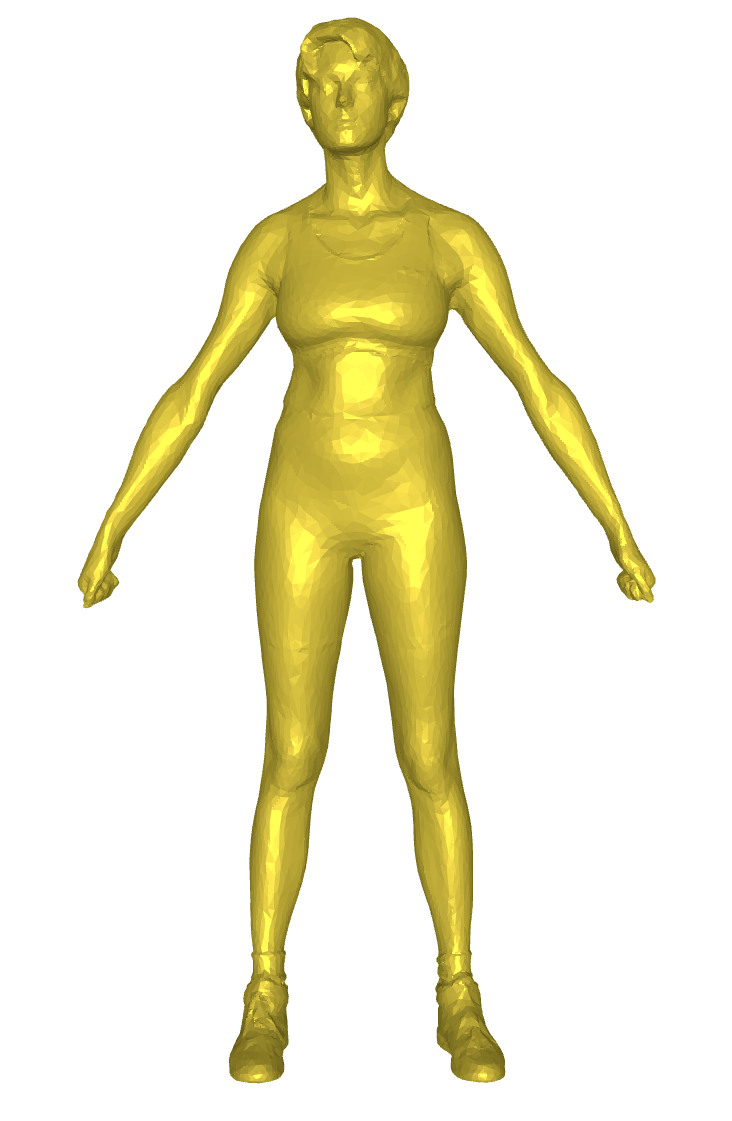
\includegraphics[width=.3\textwidth]{images/human3d.png}\hspace{0.05\textwidth}
    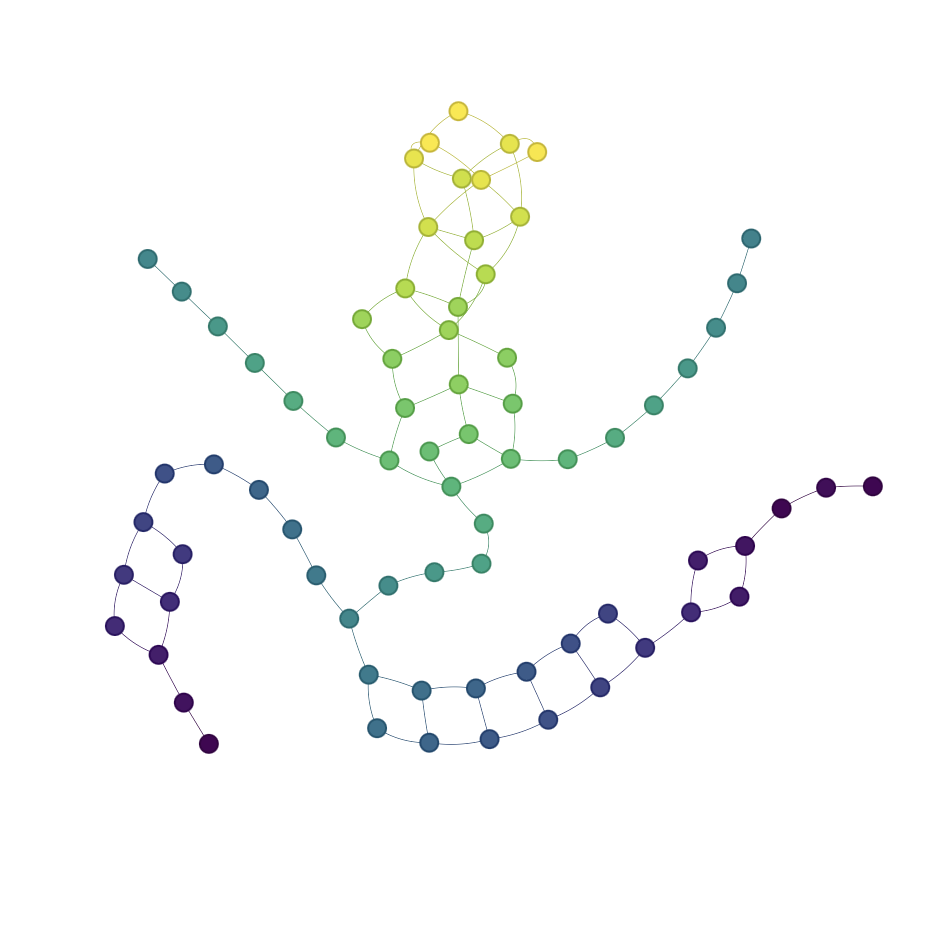
\includegraphics[width=.4\textwidth]{images/human_mapper.png}
    \caption{Left: Mesh of a $3$-dimensional point cloud representing a human shape. Right: Mapper graph computed on the point cloud using the height as filter function. Nodes are colored using the average value of the filter.}
    \label{fig:human}
\end{figure}

We then explicitly compute 2-Gromov-Wasserstein distances (as the probability measure is fixed) between different Mapper graphs on this point cloud that are obtained using the same clustering algorithm (KMeans with three clusters), the same gain $g=0.3$ and resolution $r=25$, and varying the filter function. More precisely, we use filter functions from a parametrized family $\{f_t\}_t$ defined with
$$f_t(x)=\langle x,t\cdot u+(1-t)\cdot v\rangle,$$
with $u$ and $v$ being the unit vectors associated to the horizontal and vertical directions respectively. For reference, the Mapper computed with filter function $f_0$ is displayed in Figure~\ref{fig:human}. 

In Figure~\ref{fig:ot_filter}, we plot the resulting 2-Gromov-Wasserstein distances between the Mapper graph computed with $f_0$ and the Mapper graphs computed with $f_t$ with respect to $\Vert f_0-f_t\Vert_{\infty}=\sup_{x\in\mathbb{X}}|f_0(x)-f_t(x)|$.
As one can see, the distances increase monotonically, indicating that Gromov-Wasserstein distances between Mapper graphs might be stable w.r.t. perturbations of filter functions - a theoretical direction that we aim at pursuing in future work.

\begin{figure}[t]
    \centering
    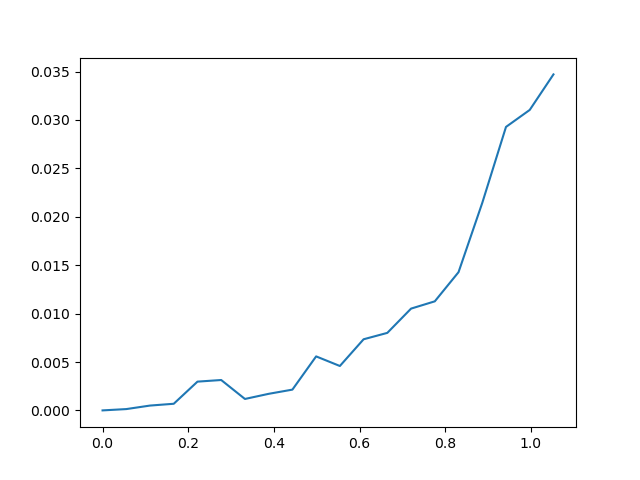
\includegraphics[width=.5\textwidth]{images/ot_filter.png}
    \caption{2-Gromov-Wasserstein distances between the Mapper graph computed with $f_0$ and the Mapper graphs computed with $f_t$ with respect to $\Vert f_0-f_t\Vert_{\infty}$.}
    \label{fig:ot_filter}
\end{figure}



\subsection{Change of measure}
In this section,
we illustrate the effect of varying the underlying probability measures, 
%that the Gromov-Wasserstein distance between Mapper graphs is sensitive to the change of measure with respect to which the sample is drawn.\\
by computing Mapper graphs on point clouds sampled from a torus $\torus$ with different probability measures. The torus $\torus$ is a two dimensional manifold that can be parametrized with two angles $(\theta,\phi)\in[0,2\pi]^2$ and can be embedded in $\R^3$ with
\begin{align*}
\embd\colon[0,2\pi]^2&\longrightarrow\R^3\\
(\theta,\phi)&\longmapsto((a+b\cos(\theta))\cos(\phi),(a+b\cos(\theta))\sin(\phi),b\sin(\theta))
\end{align*}
where $a,b>0$ are two radius parameters.
%
We use the height function $f$ as filter, which is given by the projection of $\embd$ over its first coordinate, i.e., $f\colon(\theta,\phi)\mapsto(a+b\cos(\theta))\cos(\phi)$. It can easily be checked that $f$ is a Morse function, by differentiating twice over $\theta$ and $\phi$.
%
Moreover, %$\torus$ is a Riemannian manifold by considering 
the Riemannian metric $\g$ induced by the torus embedding in $\R^3$, 
%It can be checked that $\g$ 
is given at any point $(\theta,\phi)$ by the positive definite matrix
$$\G(p)=\begin{pmatrix}
b^2 & 0 \\
0 & (a+b\cos(\theta))^2
\end{pmatrix}.$$
We will consider several probability measures $\mes_{p,q}$ on $\torus$ that are parametrized by two values $0<p,q<1$, that give the proportion of points sampled in the region $\phi\in[5\pi/6,7\pi/6]$, and the proportion in the region $\phi\in[0,\pi/6]\cup[11\pi/6,2\pi]$, respectively. More explicitly, we define
$$d\mes_{p,q}(\theta,\phi)=\frac{u_{p,q}(\phi)(a+b\cos(\theta))d\theta d\phi}{2\pi a},$$

where
$$u_{p,q}(\phi)=p\frac{3}{\pi}\ind_{[5\pi/6,7\pi/6]}(\phi)+q\frac{3}{\pi}\ind_{[0,\pi/6]\cup[11\pi/6,2\pi]}(\phi)+(1-p-q)\frac{3}{4\pi}\ind_{[\pi/6,5\pi/6]\cup[7\pi/6,11\pi/6]}(\phi).$$
Notice that the special case $p=q=1/6$ corresponds to the normalized volume measure on $\torus$.
%
We fix $a=0.75$ and $b=0.25$, and we pick values for $p$ and $q$ in the $3\times 3$ grid $[1/9,1/6,1/3]^2$, resulting in nine different probability measures. Then, we sample $n_{p,q}=2\cdot10^5$ points from each probability measure $\mes_{p,q}$, and construct the corresponding Mapper graphs $\{\mapper_{p,q}\}_{p,q}$ using resolution $r=30$ and gain $g=0.3$ for all $(p,q)$ pairs. See Figure~\ref{fig:torus} for an example of three of these samples, and Figure~\ref{fig:mapper_torus} for the corresponding Mapper graphs. %constructed using these three samples and we color the vertices and edges using their associated measure. 

First, remark that the Mapper graphs $\{\mapper_{p,q}\}_{p,q}$ are all identical as (combinatorial) simplicial complexes. %\mathieu{Ce serait bien de donner les 9 Mappers avec les noeuds / arètes coloriés par la masse correspondante.}
However, as they are different as metric measure spaces, when considering the $2$-Gromov-Wasserstein distances $\Hat{\gromov_2}$ between these metric measure spaces $\{(\mapper_{p,q},\haus,\mes_{p,q}\circ\DD^{-1})\}_{p,q}$, we  obtain a $9\times 9$ distance matrix %between the Mapper graphs 
with nonzero entries.
%exhibiting some differences. 
In order to visualize it,
%we use the Euclidean distance in $\R^3$ to compute Hausdorff distances between Mapper nodes and edges, and 
we perform multi-dimensional scaling (MDS) to visualize this distance matrix as a 2-dimensional point cloud in Figure~\ref{fig:mds}. The correspondence between the point labels in Figure~\ref{fig:mds} and the corresponding $(p,q)$ parameters  
%of the corresponding probability measure with respect to which the Mapper graph was computed 
is given in Table~\ref{tab:corr}. In Figure~\ref{fig:mds}, we can see three pairs of points, namely $(b,d)$, $(c,g)$ and $(f,h)$, that are close in the MDS representation, illustrating the fact that %This is because 
each of these pairs corresponds to two symmetric parameter pairs $(p,q)$
%of values of the  $(p,q)$, 
%and that this means that the 
that induce two symmetrical underlying probability measures on $\torus$ with respect to the vertical axis. One can also see that the points labeled $a$ and $i$, which correspond to those two measures that assign the least and the most mass in the two regions of the torus, respectively, are the ones that are the farthest away from the remaining points, indicating that the corresponding Mapper graphs computed using these two measures are the most different from the others. 

\begin{figure}[H]
    \centering
    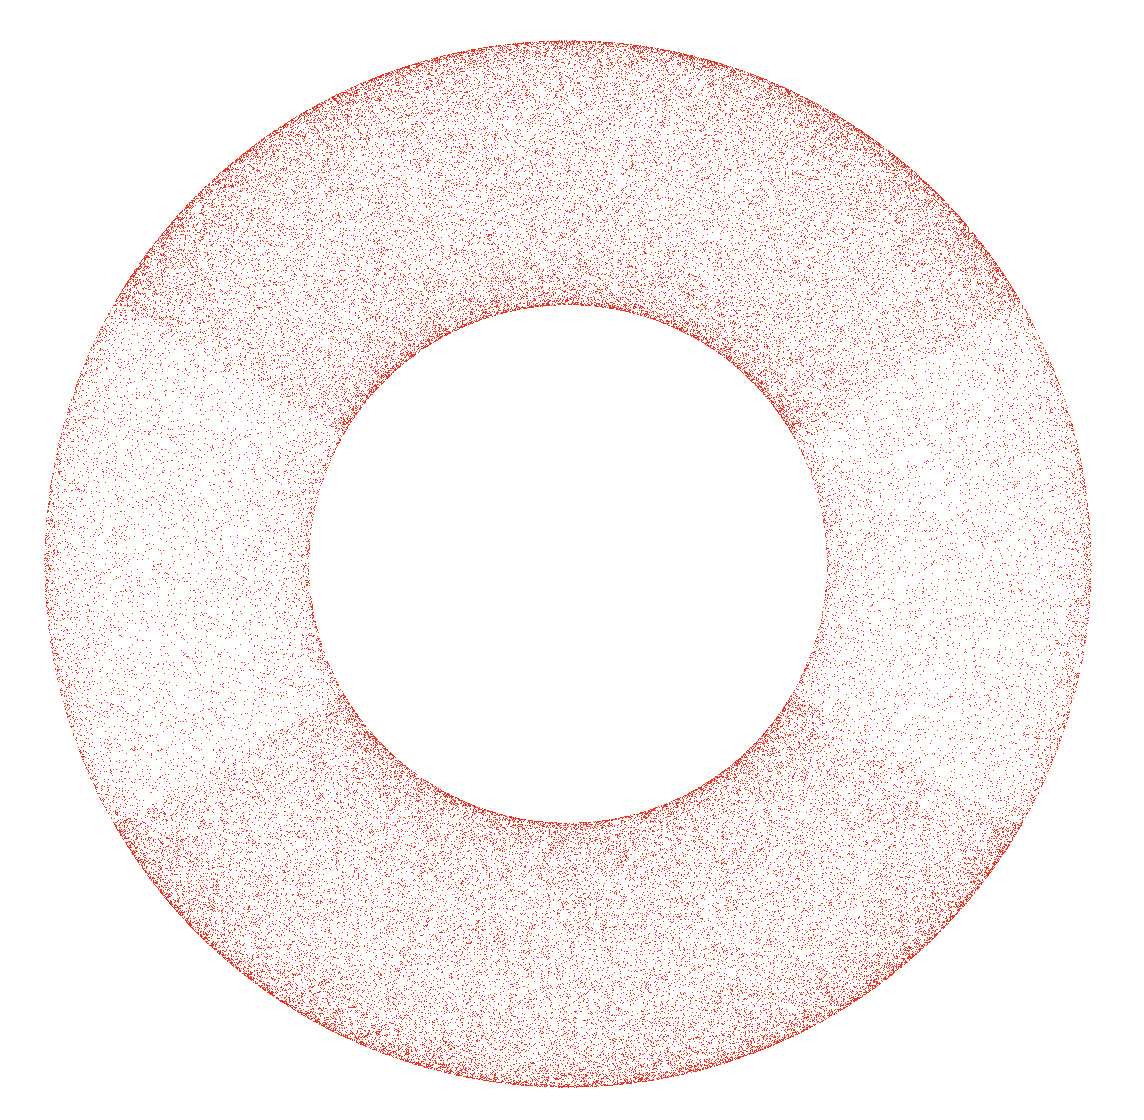
\includegraphics[width=.25\textwidth]{images/torus112.png}\hspace{0.05\textwidth}
    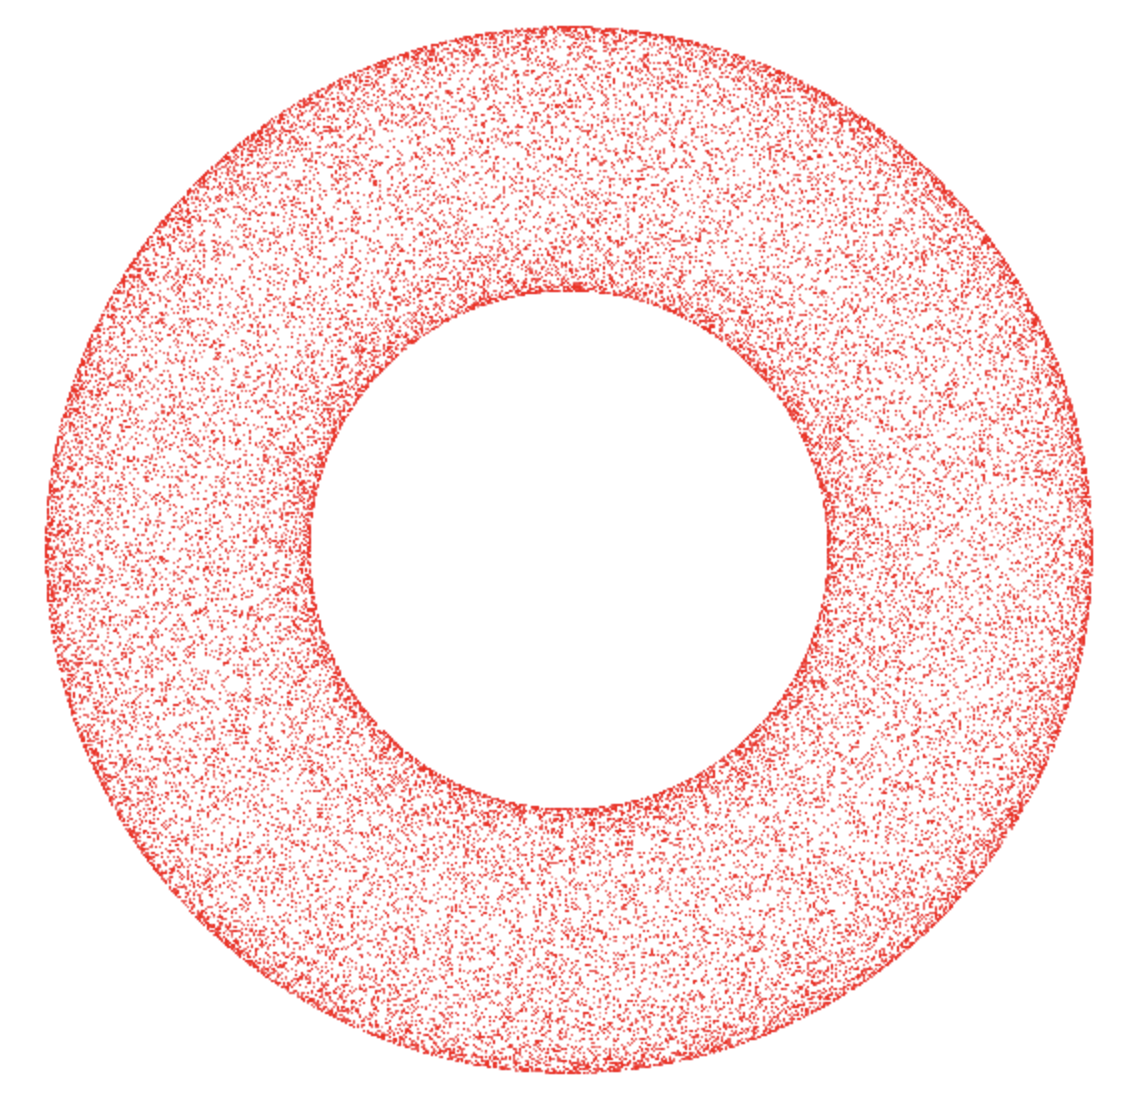
\includegraphics[width=.25\textwidth]{images/torus16.png}
    \hspace{0.05\textwidth}
    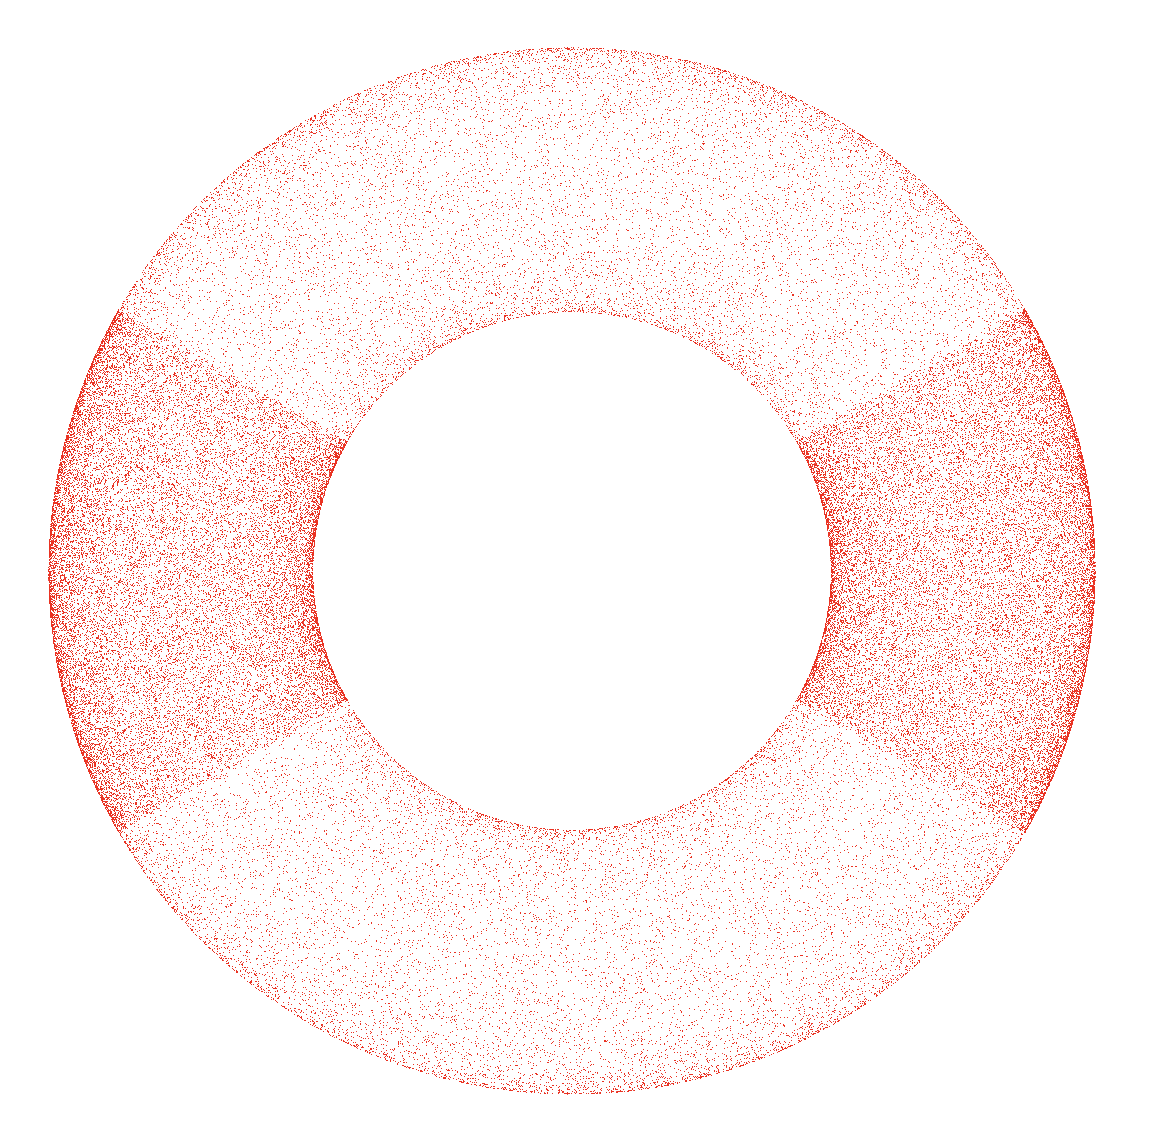
\includegraphics[width=.25\textwidth]{images/torus13.png}
    \caption{Point clouds sampled from $\mes_{p,q}$ for different values of $p$ and $q$. Left: $p=q=1/12$. Middle: $p=q=1/6$ (uniform measure). Right: $p=q=1/3$.}
    \label{fig:torus}
\end{figure}

\begin{figure}[H]
    \centering
    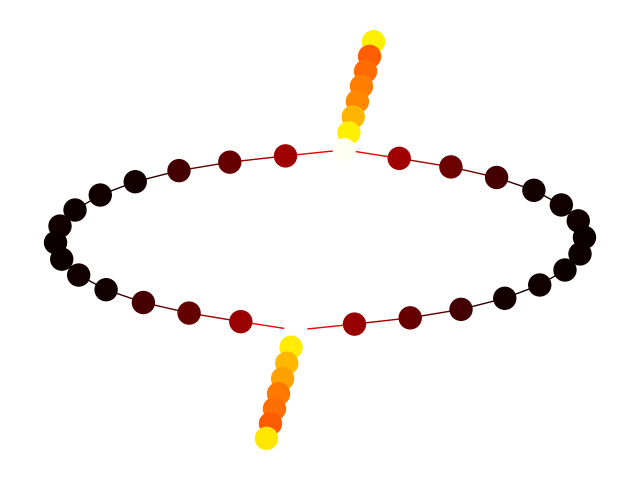
\includegraphics[width=.25\textwidth]{images/mapper12.png}\hspace{0.05\textwidth}
    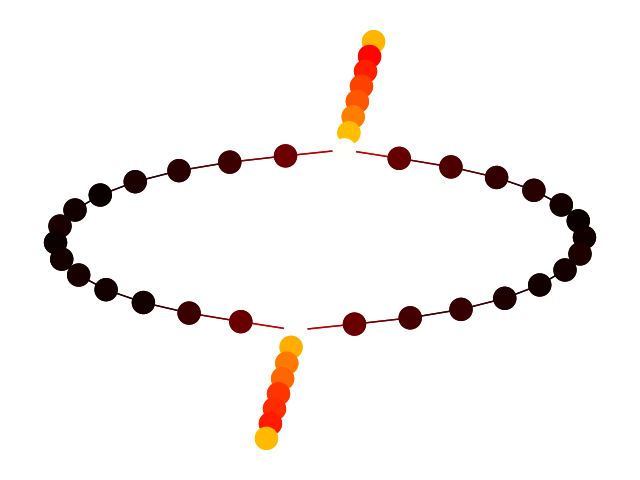
\includegraphics[width=.25\textwidth]{images/mapper16.png}
    \hspace{0.05\textwidth}
    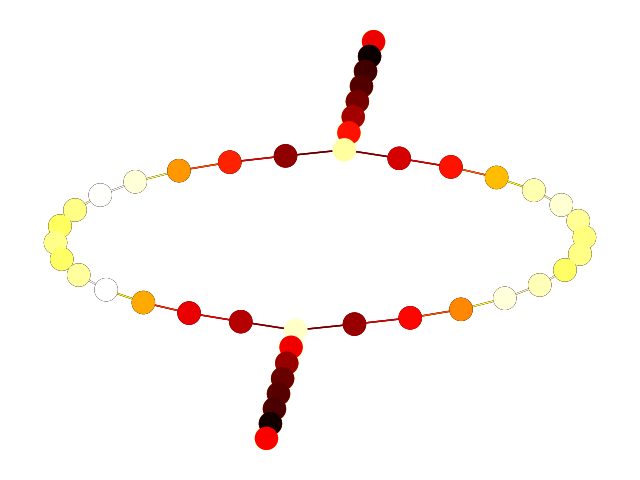
\includegraphics[width=.25\textwidth]{images/mapper13.png}
    \caption{Mapper graphs computed on the samples shown in Figure~\ref{fig:torus}. Vertices and edges are colored using their associated masses. Left: $p=q=1/12$. Middle: $p=q=1/6$ (uniform measure). Right: $p=q=1/3$.}
    \label{fig:mapper_torus}
\end{figure}
\begin{figure}[H]
    \centering
    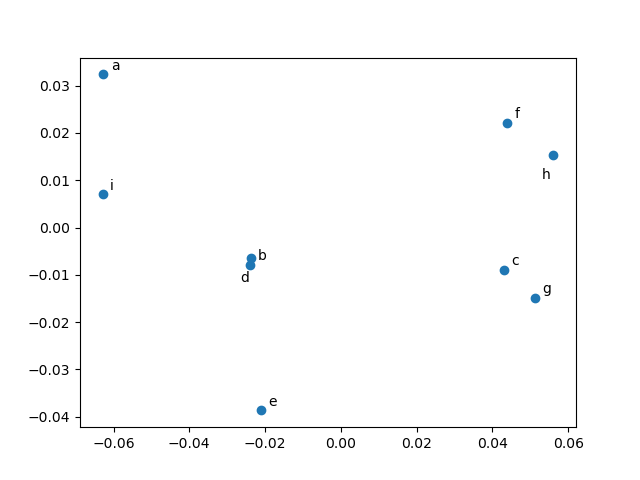
\includegraphics[width=.5\textwidth]{images/mds.png}
    \caption{MDS visualization of the Gromov-Wasserstein distance matrix between the different Mapper graphs.}
    \label{fig:mds}
\end{figure}

\begin{table}[H]
\begin{center}
\begin{tabular}{ |c|c|c| } 
 \hline
 Label & p & q \\
 \hline
 a & 1/12 & 1/12 \\ 
 \hline
 b & 1/12 & 1/6 \\ 
 \hline
 c & 1/12 & 1/3 \\ 
 \hline
 d & 1/6 & 1/12 \\ 
 \hline
 e & 1/6 & 1/6 \\ 
 \hline
 f & 1/6 & 1/3 \\ 
 \hline
 g & 1/3 & 1/12 \\ 
 \hline
 h & 1/3 & 1/6 \\ 
 \hline
 i & 1/3 & 1/3 \\ 
 \hline
\end{tabular}
\caption{Correspondence between the labels of Figure~\ref{fig:mds} and the parameters of $\mes_{p,q}$.}
\label{tab:corr}
\end{center}
\end{table}














 